% ---------------------------------------------------------------------------
% Author guideline and sample document for EG publication using LaTeX2e input
% D.Fellner, v1.13, Jul 31, 2008

\documentclass{egpubl}
\usepackage{eurovis2018}
\STAR_Eurovis
% --- for  Annual CONFERENCE
% \ConferenceSubmission   % uncomment for Conference submission
% \ConferencePaper        % uncomment for (final) Conference Paper
% \STAR                   % uncomment for STAR contribution
% \Tutorial               % uncomment for Tutorial contribution
% \ShortPresentation      % uncomment for (final) Short Conference Presentation
% \Areas                  % uncomment for Areas contribution
% \MedicalPrize           % uncomment for Medical Prize contribution
% \Education              % uncomment for Education contribution
%
% --- for  CGF Journal
% \JournalSubmission    % uncomment for submission to Computer Graphics Forum
% \JournalPaper         % uncomment for final version of Journal Paper
%
% --- for  EG Workshop Proceedings
% \WsSubmission    % uncomment for submission to EG Workshop
% \WsPaper         % uncomment for final version of EG Workshop contribution
%
\electronicVersion % can be used both for the printed and electronic version

% !! *please* don't change anything above
% !! unless you REALLY know what you are doing
% ------------------------------------------------------------------------

% for including postscript figures
% mind: package option 'draft' will replace PS figure by a filname within a frame
\ifpdf \usepackage[pdftex]{graphicx} \pdfcompresslevel=9
\else \usepackage[dvips]{graphicx} \fi

\PrintedOrElectronic

% prepare for electronic version of your document
\usepackage{t1enc,dfadobe}

\usepackage{egweblnk}
\usepackage{cite}

\usepackage{comment}
\usepackage[ngerman]{babel}
\usepackage[utf8]{inputenc}
\usepackage[T1]{fontenc}
\usepackage{amsmath}
\usepackage{graphicx}
\usepackage{listings}
\usepackage{tabularx}
\usepackage{hyperref}
\usepackage[autostyle]{csquotes}  

\newcommand{\pvec}[1]{\vec{#1}\mkern2mu\vphantom{#1}}

%opening
%\title{Survey of Vascular Visualization Techniques}
%\author[C. Br{\"a}ndle \& N. Leopold]{Christian Br{\"a}ndle and Niko Leopold\\TU Vienna\\}

\title{Project Report: Direct Volume Rendering Techniques for Cardiovascular Visualization} 
%\subtitle{Visualization of Medical Data 2, 2017W} 
\author{Christian Br{\"a}ndle \& Niko Leopold \\ Visualization of Medical Data 2, 2017W}


\begin{document}

\graphicspath{{images/}}

\maketitle

\keywords{Cardiovascular visualization, direct volume rendering, raytracing, transfer function design, intensity projection, curviplanar reformation, geometric modeling, vascular system modeling, convolution surfaces, implicit modeling, vessel reconstruction method, level sets, quad dominant meshes}

\begin{abstract}
%	The visualization of cardiovascular structures is an essential aspect of 
%    the diagnostic process therapy planning. This survey provides an overview
%    over recent advances in both model-free and model-based vascular visualization techniques.
%    In the field of direct volume rendering, the focus is on advanced transfer function design to         
%	highlight abnormalities of the vessel wall, as well as providing aggregated rotation independent
%	2D projections and depth cues for effective diagnosis.
%	Furthermore, improved model-based techniques are discussed, which provide 
%	more accurate and effective sceletonization and surface reconstruction.
		
	\begin{classification} % according to http://www.acm.org/class/1998/
		\CCScat{Computer Graphics}{I.3.3}{Picture/Image Generation}{};
		\CCScat{Computer Graphics}{1.3.7}{Three-dimensional Graphics and Realism}{};
		\CCScat{Computer Graphics}{1.3.5}{Computational Geometry and Object Modeling}{};
		%\CCScat{Computer Graphics}{I.3.3}{Mesh, parametrization}{}
	\end{classification}
	
\end{abstract}

%-------------------------------------------------------------------------
\section{Motivation}

In the STAR report we have discussed various techniques related to the visualization of cardiovascular structures. We have covered both model-based and model-free approaches. Model-based mesh generation follows some more restrictive assumptions about the vascular structure whereas model-free methods such as direct volume rendering tries to capture as much original information as possible. Model-based techniques are often used for treatment planning and basic anatomical overview, whereas model-free methods are required for precise diagnostics.

We decided that for the project implementation we wanted to focus on direct volume rendering. The goal was to effectively visualize thin vessel structures and if possible even their narrowings due to stenoses etc. At first we considered to implement the automatic transfer function specification for visual emphasis of coronary artery plaque by Glasser et al.~\cite{glasser2010automatic}. However we realized that due to time constraints this would not be possible as it involves a large number of different pipelines stages. We thus decided to implement instant volume visualization using \emph{Maximum Intensity Difference Accumulation} (MIDA) by Bruckner and Gr{\"o}ller~\cite{bruckner2009instant}.


% \section{Related Work}

%-------------------------------------------------------------------------
%\section{Data}
\section{DICOM Data}

To visualize cardiovascular data we first had to search approprite data that exhibit the information we want to visualize.

%\subsection{DICOM}

In the field of medical visualization DICOM is the defacto standard for capturing, annotating and deploying data.
Including meta information and high dynamic range images DICOM is our preferred way to load medical data into our system.

\subsection{Data Acquisition}

To our disappointment we had to find out that it is rather difficult to find appropriate vascular data of the heart.


\subsection{Data Import}

One of the key advantages of DICOM data over simple image stacks is the fact that pixel intensities and radiometric intensities do not need to be the same in a given image stack. So DICOM provides a mapping to use several images together within a homogen radiometric background.


\begin{figure}[h]
	\centering
	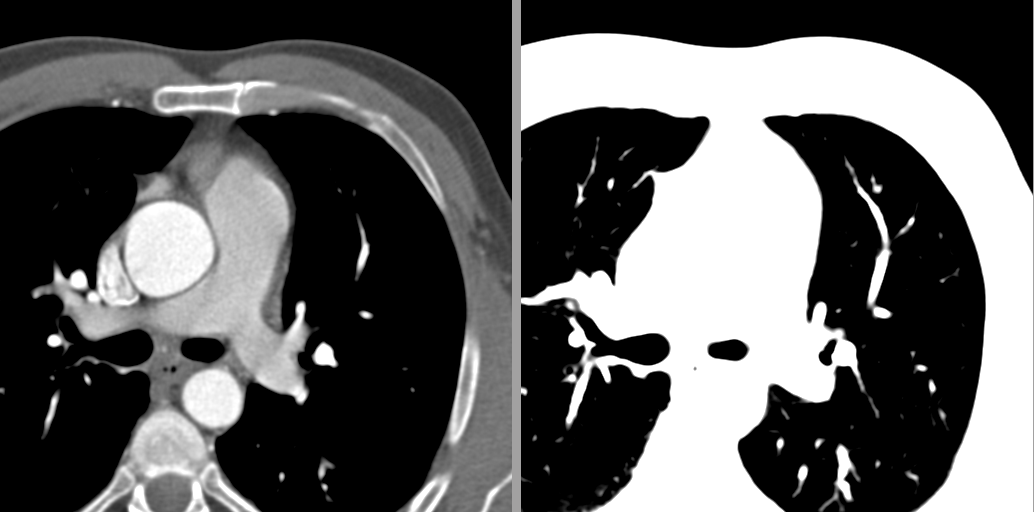
\includegraphics[width=0.45\textwidth]{IM-0001-0019_20.png} \\
	\caption{Stacked images with inhomogenous radiometric space. DIOCM sample data \emph{CARDIX} \cite{gimias_sampledata_2018} aquired from sample data section of the GIMAIS project \cite{gimias_2018} and processed with \emph{dicom2jpeg} from imbera project \cite{imebra_dicom_sdk_2018}.}
	\label{fig:IM-0001-0019_20}
\end{figure}

Simple exports of JPEG data out of DICOM without respecting this relation spills out images with are not homogenous across the stack as seen for instance in figure \ref{fig:IM-0001-0019_20}.


\subsection{Data Conversion}

As it was not possible to find a suitable DICOM reader for our \emph{CARDIX} dataset \cite{gimias_sampledata_2018} for VTK we used an intermediate step via MITK and convert DICOM data with the help of MITK main application to VTK 3D Image (VIK) data readable by VTK.
In this way we could overcome the problems with codecs and intensity differences across the image stack.




%-------------------------------------------------------------------------
\section{Medical Visualization System}

As our original goal was to use an existing application and enhance it with certain abilities we researched the web to find open source applications that are cross platform and run under Windows and Linux environments.
As this is a quite restrictive approach we actually found a lot more applications and frameworks but exclude them for the reasons above.

Our search continued then with frameworks as we saw that there was no application that fulfilled our needs and was capable for rapid prototyping our system.
With frameworks we unfortunately also didn't have more luck as the way the frameworks limit us in regards of data import and data visualization was as well not suitable to develop our chosen algoritm rapidly.

In the end we utilize an OpenGL based visualion project to implement our algorithm there. Additional libraries to load DICOM data were searched but also there we experience several problems with codecs for instance.

%\section{Applications}
%
%% Surface Visualization Apps?

\subsection{3DSlicer}

\blockquote{3D Slicer is an open source software platform for medical image informatics, image processing, and three-dimensional visualization \cite{3DSlicer_2018}.}

The power of 3DSlicer lies in the handy user interface and the amount of resources how to deal with the program. Also youtube is a good source and this is how we lernt to do some basic tasks with 3DSlicer. It can also import several kinds of DICOM data, which is a prerequisite for our medical visualization application.

Although very nice at user level we do not discover a developer guide that assists us well through the internals of 3DSlicer.
As our goal was not to use the application but rather to implement renderers for example we hadn't the impression that this would be possible in reasonable amount of time.

%\subsubsection{\emph{MAGIX} Dataset in 3DSlicer}

\begin{figure}[h]
	\centering
	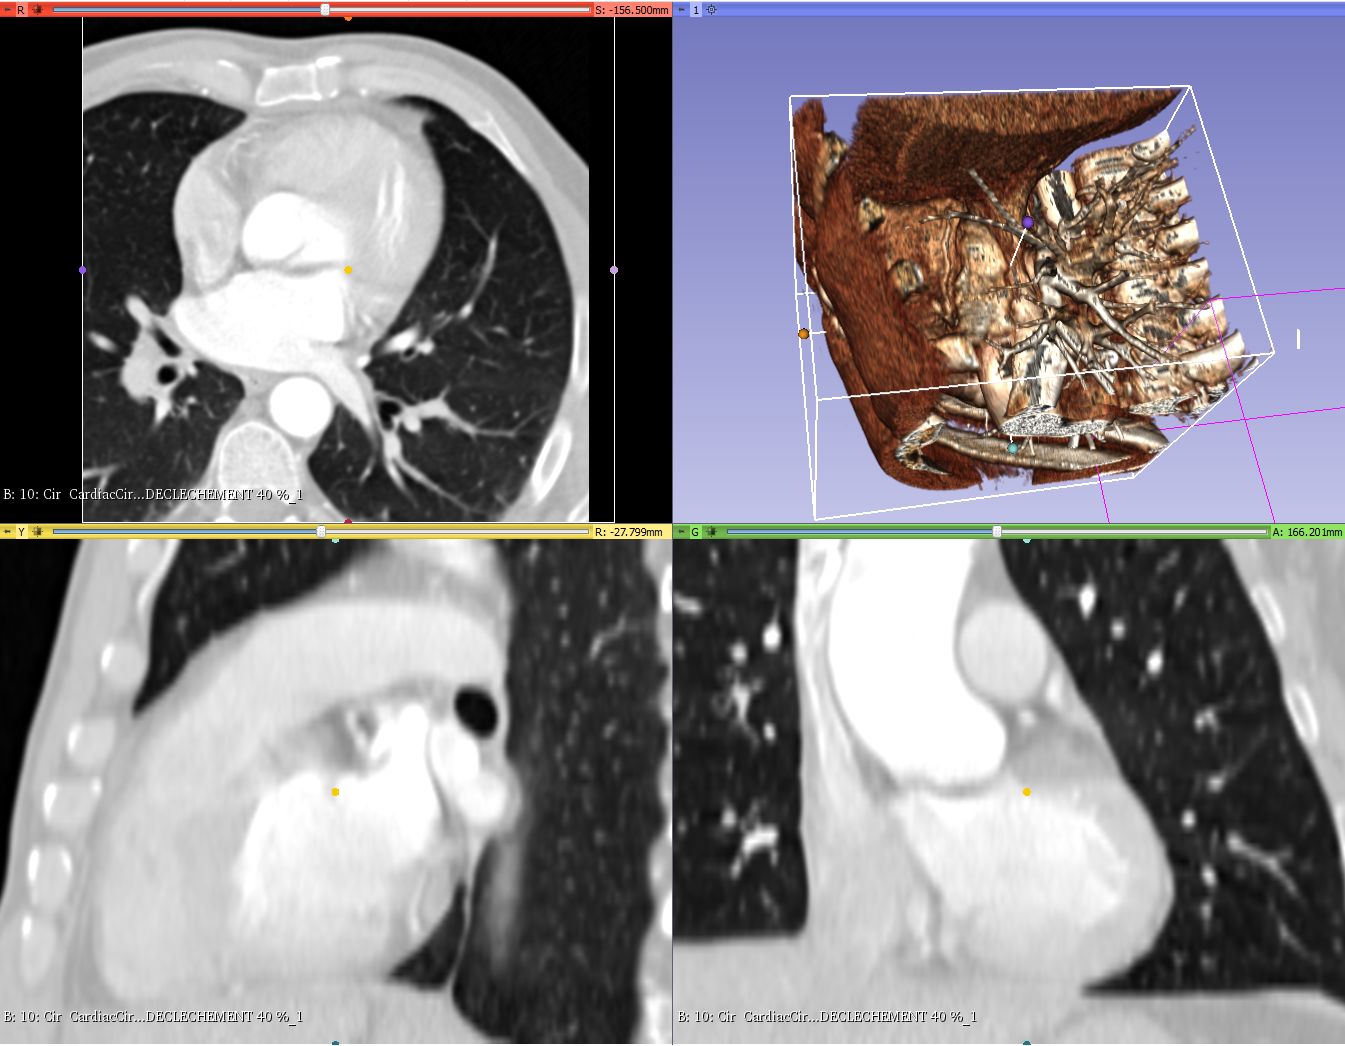
\includegraphics[width=0.45\textwidth]{Slicer3D_MAGIX_01.png} \\
	\caption{ \emph{MAGIX}\cite{gimias_sampledata_2018} dataset visualized with \emph{Slicer3D}.}
	\label{fig:Slicer3D_MAGIX_01}
\end{figure}

As could be seen in figure \ref{fig:Slicer3D_MAGIX_01}, we visualized one of our example datasets, \emph{MAGIX} with volume rendering provided by 3DSlicer.


\subsection{MITK - The Medical Imaging Interaction Toolkit}

\blockquote{The Medical Imaging Interaction Toolkit (MITK) is a free open-source software system for development of interactive medical image processing software. MITK combines the Insight Toolkit (ITK) and the Visualization Toolkit (VTK) with an application framework \cite{MITK_2018}.}

In comparison to 3DSlicer MITK offers a better developer documentation and a description of the internal structure of MITK. Further it supplies guides how to create plugins or template based-projects that help to develop own applications with the MITK framework. Build instructions and a description of the render concept concludes our decision to take a closer look at this open source project.
Also DICOM loaders are integrated and we managed to visualize one of our demo datasets in MITK. A downside was the stability of MITK as it happened several times that the application crashed after selecting DICOM data for volumetric visualization.

% TODO: add ref to chapter
As we are interested in writing an own renderer and as MITK uses VTK to visualize data, we refer here to the VTK section that describes our experience with VTK in more detai.

%\subsubsection{MITK Plugin}

%\subsubsection{\emph{CARDIX} Dataset in MITK}

\begin{figure}[h]
	\centering
	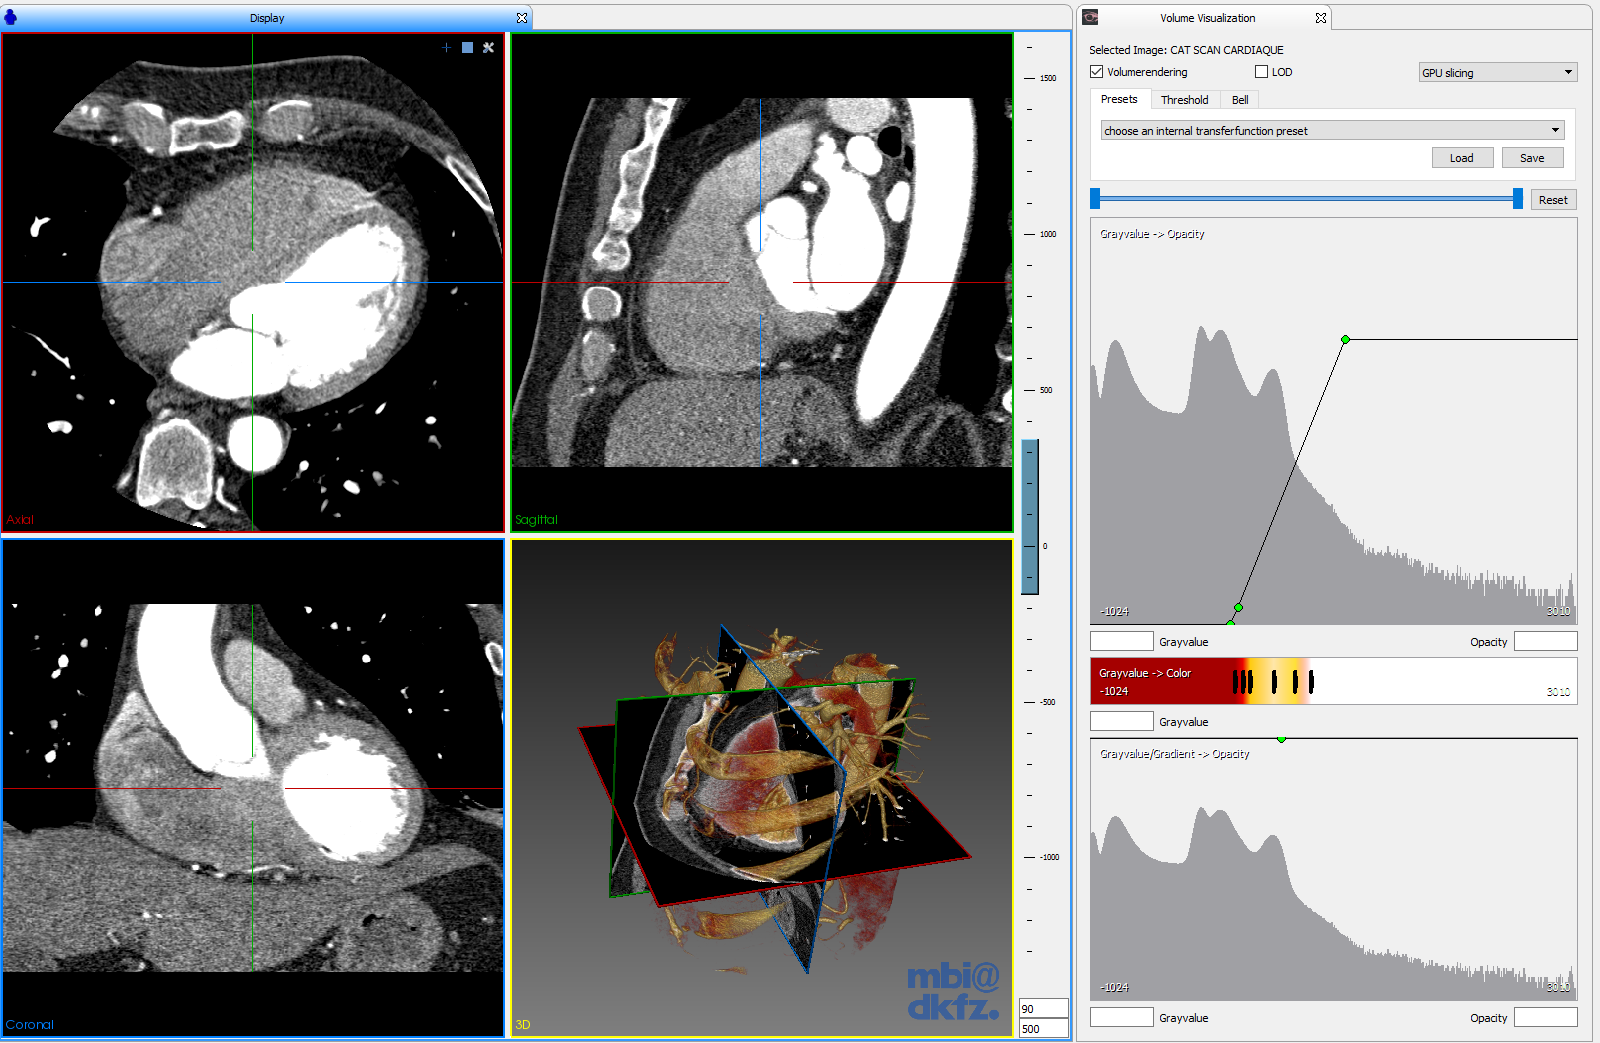
\includegraphics[width=0.45\textwidth]{MITK_CARDIX_01.png} \\
	\caption{ \emph{CARDIX}\cite{gimias_sampledata_2018} dataset visualized with \emph{MITK}.}
	\label{fig:MITK_CARDIX_01}
\end{figure}

As could be seen in figure \ref{fig:MITK_CARDIX_01}, we visualized one of our example datasets, \emph{CARDIX} with volume rendering provided by the MITK application.

%\section{Frameworks}

\subsection{VTK - The Visualization Toolkit}

\blockquote{The Visualization Toolkit (VTK) is an open-source, freely available software system for 3D computer graphics, image processing, and visualization. It consists of a C++ class library and several interpreted interface layers including Tcl/Tk, Java, and Python. VTK supports a wide variety of visualization algorithms including scalar, vector, tensor, texture, and volumetric methods, as well as advanced modeling techniques such as implicit modeling, polygon reduction, mesh smoothing, cutting, contouring, and Delaunay triangulation. VTK has an extensive information visualization framework and a suite of 3D interaction widgets \cite{vtk_2018}.}

As VTK was the central part of actual all medical visualization toolkits researched we wanted to use this framework for our application.
Our resources for learning VTK were \emph{The Visualization Toolkit}\cite{schroeder2004visualization}, \emph{The VTK Users's Guide}\cite{avila2010vtk} and of course the VTK webpage \cite{vtk_2018}.

Several parts of the VTK chain were researched, as there are:

\subsubsection{Loading Data with VTK Readers}
%\subsubsection{VTK Reader}

VTK also supports to load DICOM data via specific VTK Readers. As our data is formed of DICOM files we take a closer look at that feature. Unfortunately due to problems with the codec included in our DICOM data we were not able to load the data as we want to. As we haven't found a solution to fix this we come up with a preconversion step of DICOM data with MITK, as there it is possible to save DICOM data into a VTK 3D image.  


\subsubsection{Processing Data with VTK Filters}

The VTK way of processing data is through VTK Filters. The philosophy is that filters transform or combine data within a chain or network of coupled filters that finally provide an output to one or more VTK Mappers.
To implement our direct volume rendering approach the only easy way would have been to dynamically adapt our DICOM data according to the settings of MIDA and the current view direction and further use a built-in volume renderer like RayCast Mapper to visualize the result.
As we would have to implement somehow a reverse version of MIDA and as the data transformation would have been a seperate step in the processing chain we decided not to use VTK Filters at all.

\subsubsection{Render Data with VTK Mappers}

In VTK renderer are called Mappers as they provide the ability to map a given dataset to a given device. While it is possible to override specific Mappers it is not straight forward to interfere with the renderer at OpenGL-level. 

For this reason VTK introduced VTK shaders, that are based on structured OpenGL shaders. While this give access to GLSL shaders the structure of the shaders have to follow the VTK guidelines. That include string replacement of VTK specific shading commands within the OpenGL shader.

As we haven't found appropriate information on what for string replacements exist, how they should be used and how they interact with the rest of the VTK application we decided not to use an OpenGL shader based on the VTK framework.

\subsubsection{VTK Example Application}

\begin{figure}[h]
	\centering
	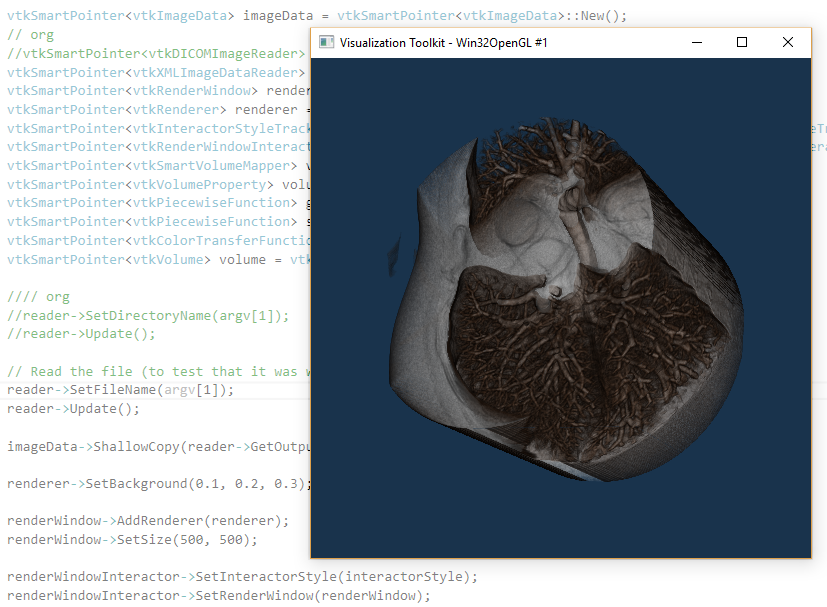
\includegraphics[width=0.45\textwidth]{VTK_Image_Renderer_02_II.png} \\
	\caption{ \emph{CARDIX} \cite{gimias_sampledata_2018} dataset rendered from VTI file with VTK Raycast Mapper.}
	\label{fig:VTK_Image_Renderer_02_II}
\end{figure}

As VTK prodides a lot of examples and tutorials on the usage of its framework we gave it a try and load a 3D image in form of a VTI file into a simple raycaster visualization. In figure \ref{fig:VTK_Image_Renderer_02_II} we see the \emph{CARDIX} \cite{gimias_sampledata_2018} dataset visualized with this base fazilities. As VTK also provide a script interface we also build $Tcl/Tk$ and tried the same visualization on a script base, which works perfectly fine. But as already stated before we left VTK behind as it does not support an easy integration of own OpenGL shaders.

%\subsection{MITK Plugin}

%\section{Library}

% Surface Visualization Libs ?

%\subsection{DICOM Reader}

\subsection{Imbera DICOM Reader}

%Imebra: a C++ Dicom library

\blockquote{Imebra SDK is an open source C++ library that handles DICOM network messages and DICOM files \cite{imebra_dicom_sdk_2018}.}

While Imbera seems to be the library we searched for to easily read DICOM data on multiple platforms in practice it fails because of the codec used in our \emph{CARDIX} dataset. We don't know if this is due to the open source version used as we haven't tried the commercial version instead and will leave this as an open point.

%\subsection{VTK Reader}

\subsection{OpenGL Application}

As stated before we considered using the VTK (Visualization ToolKit) framework as well as the MITK (Medical Imaging Interaction Toolkit) framework. However we soon realized that it is hard to implement a custom volume renderer in these frameworks, and thus decided to fall back to our own implementation. For this we reused an old Qt framework from the vis1 course that had simple GPU direct volume rendering implemented with simple alpha compositing, but with no proper interaction, no transfer functions and no shading.

The goal was to extend this framework with
\begin{itemize}
	\item More compositing methods: Maximum Intensity Projection (MIP), Minimum Intensity Projection (MINIP), Average Intensity Projection (AIP) as well as Maximum Intensity Difference Accumulation (MIDA)
	\item Interactive controls
	\item Gradient-based shading
	\item Customizable transfer functions
\end{itemize}

%\section{MIDA Processing Chain}

% Surface Visualization Chain ?
% MIDA Chain
% To process our data with MIDA we utilize VTK and use its VTI ...

%\section{MIDA Algorithm}

\section{MIDA  - Maximum Intensity Difference Accumulation}

MIDA is a compositing technique for Direct Volume Rendering (DVR) and was first published from Bruckner et al.~\cite{bruckner2009instant}.
It combines the advantage of Maximum Intensity Projection (MIP), where important structure shine through all data, 
with the advantage from traditinal DVR, where depth cues stem from color and opacity accumulation.

The advantages and disadvantagesof the combined technologies are more precisely:

\begin{itemize}
\item Maximum Intensity Projection (MIP) \\
+ MIP does not require a transfer function .\\
- The spatial context in MIP visualization is lost as the most important pixel just shine trough. \\
\item Direct Volume Rendering (DVR)\\
+ DVR accumulates color and opacity, it uses mostly gradient-based shading. \\
- Shading have to interpolate between unshaded and gradient-based shading according to gradient magnitude. \\ 
- DVR needs appropriate transfer function, otherwise crucial information won't be visualized well 
  and important features will disapear in fog or will be occluded by unimporant data.
\end{itemize}

\subsection{MIDA - Accumulation}
\label{sec:Accumulation}

MIDA is rendered with front-to-back traversal order.  
It focus the interest on the regions of a ray where the maximas are and values change from low to high. The amount of change is represented by $\delta_i$ for the $i$th sample position $P_i$ along the ray and $f_{max_i}$ represents the current maximum found.
MIDA overrides the occlusion relationship of the previous accumulated color $c_i$ and opacity $\alpha_i$ when a new maximum is encountered, where the weights are defined by $beta_i$.

\begin{eqnarray}
%\begin{aligned}
\delta_i = & \begin{cases}
f_{P_i} - f_{max_i}, & \text{if $f_{P_i} > f_{max_i}$}\\
0, & \text{otherwise}
\end{cases} \\
\beta_i = & 1 - \delta_i \\
c_i = & \beta_i c_{i-1} + (1 - \beta_i \alpha_{i-1}) \alpha(f_{P_i})c(f_{P_i}) \\
\alpha_i = & \beta_i \alpha_{i-1} + (1 - \beta_i \alpha_{i-1}) \alpha(f_{P_i}) 
%\end{aligned}
\label{eqn:MIDA}
\end{eqnarray}

It has to be noted that color $c_i$ and opacity $\alpha_i$ are computed the same way as for normal DVR, except that there is the additional weighting with $\beta_i$, see equation \eqref{eqn:MIDA}.

\subsection{MIDA - Interpolation}

MIDA can interpolate between it's two extremes, namely DVR and MIP in a continuous fashion.
To achieve this a interpolation variable $\gamma$ is defined that ranges from $-1$ to $1$, i.e. $\gamma=[-1,1]$.
As interpoaltion is different in the direction of DVR compared to the direction of MIP we treat each case accordingly. 

\subsubsection{MIDA to DVR}
\label{seq:MIDAtoDVR}

As explained in section~\ref{sec:Accumulation} interpolation is done in 3D domain. It is based on the modulation of previously accumulated color and opacity. As $\gamma$ moves from MIDA to DVR we adjust the value of $\beta$ accordingly.

\begin{equation}
	\begin{aligned}
	\beta_i = & \begin{cases}
	1 - \delta_i (1 + \gamma), & \text{if $\gamma < 0$}\\
	1 - \delta_i, & \text{otherwise}
	\end{cases} \\
	\end{aligned}
\label{eqn:MIDAtoDVR}
\end{equation}

In that way equation \eqref{eqn:MIDAtoDVR} smoothly fade out high intensity values while $\gamma$ is reduced.

\subsubsection{MIDA to MIP}

Because regions of interest would be 'thinned' to just only one value shading in 3D domain would lead to artifacts when $\gamma$ is arriving at a value of $1$.
So in contrast to section~\ref{seq:MIDAtoDVR} interpolation here is done in image domain between color and opacity values of MIDA and color and opacity values of MIP. 


\subsection{MIDA - Shading \& Classification}

As shading expose artifacts if it is based on gradient directions with low magnitude like gradients from noise, the magnitude of gradient is used to interpolate between shaded and unshaded color.

To classify, separate, highlight or point out certain parts of the dataset uses simple transfer functions.
The used kind of transfer function is limited to brightness and contrast adjustment using the common window/level approach.
Alternatively users can also selct values from color maps or the like if they have preferences on that.


\section{Example Renderings}

Here we want to list some example renderings that show the capability of MIDA.

\begin{figure}[h]
	\centering
	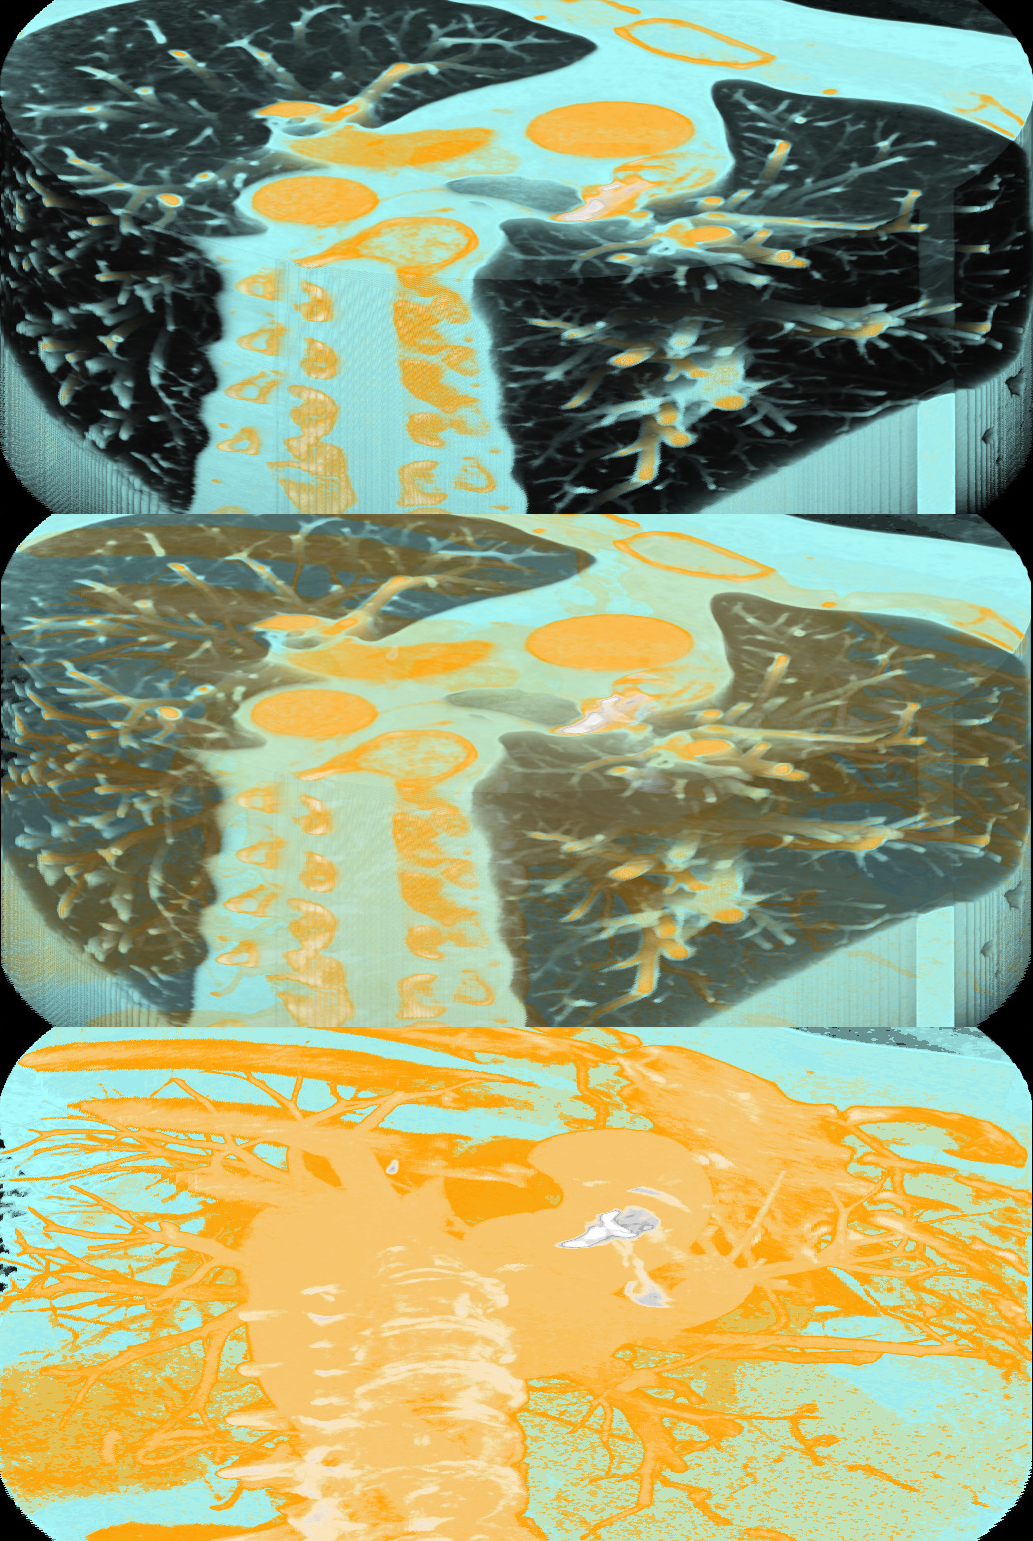
\includegraphics[width=0.35\textwidth]{MIDA_CARDIX_03.png} \\
	\caption{ \emph{CARDIX}\cite{gimias_sampledata_2018} dataset visualized with \emph{MIDA}. From top to bottom: DVR, MIDA, MIP.}
	\label{fig:MIDA_CARDIX_03}
\end{figure}


\begin{figure}[h]
	\centering
	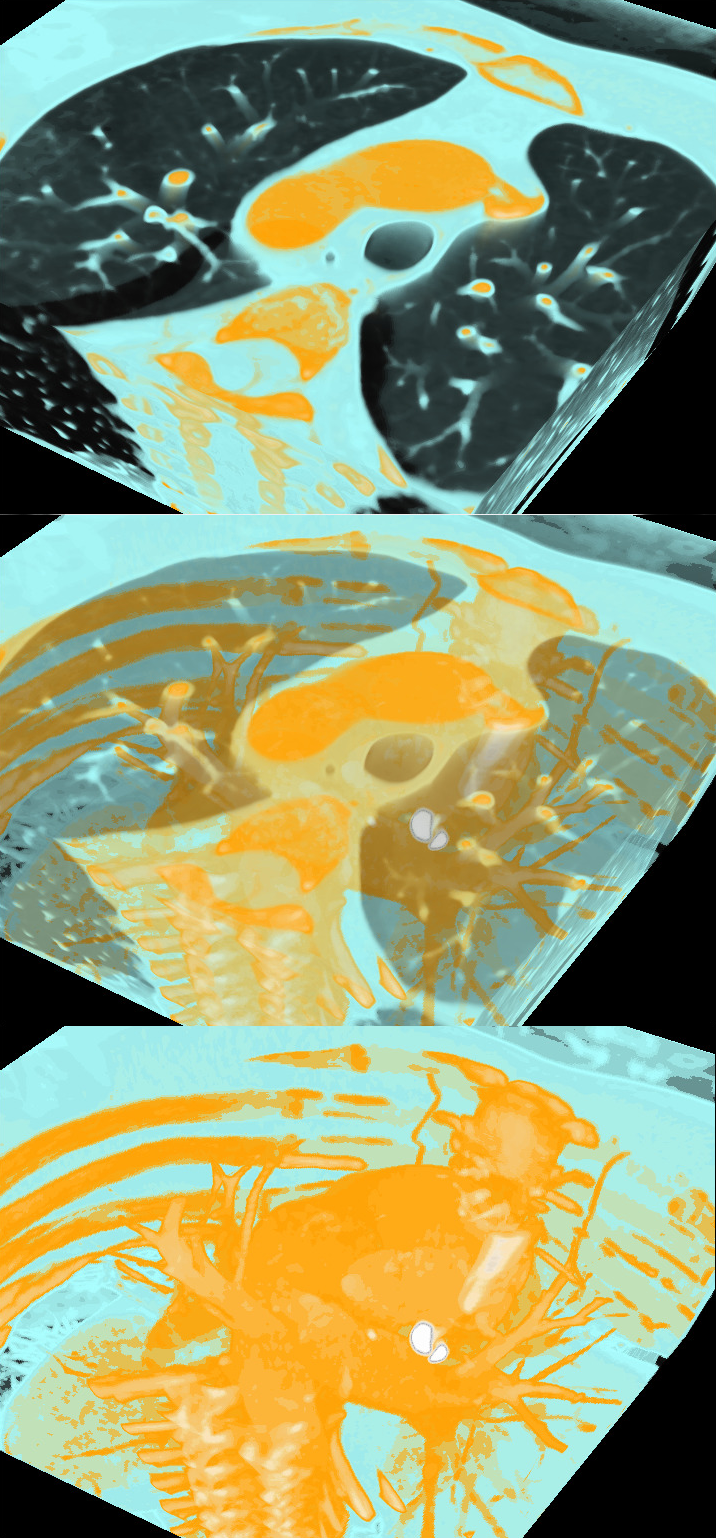
\includegraphics[width=0.35\textwidth]{MIDA_MAGIX_02.png} \\
	\caption{ \emph{MAGIX}\cite{gimias_sampledata_2018} dataset visualized with \emph{MIDA}. From top to bottom: DVR, MIDA, MIP.}
	\label{fig:MIDA_MAGIX_02}
\end{figure}

In figure \ref{fig:MIDA_CARDIX_03} and \ref{fig:MIDA_MAGIX_02} we can see the advantage of MIDA compared to DVR and MIP rendering. MIDA highlights important structures while not loosing a feeling of depth in the corresponding images.

\begin{figure}[h]
	\centering
	\includegraphics[width=0.45\textwidth]{MIDA_Angio_02.png} \\
	\caption{ \emph{Angio}\cite{gimias_sampledata_2018} dataset visualized with \emph{MIDA}. For each picture different transfer function settings are used.}
	\label{fig:MIDA_Angio_02}
\end{figure}

Figure \ref{fig:MIDA_Angio_02} shows several transfer function settings at the same MIDA-level. As seen certain coloring greatly enhance the visual perception of blood vessels and seperate them better from background information.


%-------------------------------------------------------------------------
\section{Conclusion}

The lessons learned from \emph{Medical Visualization 2} were mainly about carefull considerations necessary when using a framework.
While for a regular project the usage of a framework will pay off soon, it is different for a project of this size.

First we were enthusiastic using applications made for medical visualization like \emph{3DSlicer} and \emph{The Medical Imaging Interaction Toolkit} (MITK). Their features are tremendous and they also provide possibilities to infer with the program at script or code level. There also exists nice dialogs for interation, like transfer function dialogs and the like.
But the structure of the applications also limit the flexibility of what can be implemented and how it has to be implemented.
We were not able to implement our OpenGL rendering algorithm in such a framework without spending too much time in understanding the internals for the system. While this doesn't mean that it is impossible to extend the rendering capabilities of those applications we are confinced that we would have spent too much time on understanding the internals and therefore that this track is too dangerous with our deadline in mind. 

Then we inspect the \emph{Visualization ToolKit} (VTK), actually for two reasons. First VTK is the integral part of more or less all medical visualization applications observered and second VTK itself is also a good starting point for crafting own visualization applications.
But soon we realized that also in VTK it is difficult to implement an own OpenGL-based renderer. More suitable for modifying data in a chain or netowrk of filters, VTK also put heavy restrictions on the creation of OpenGl-based renderers. The elements that should be used in a VTK OpenGL renderer are strings that are replaced internally to assemble a final version of the OpenGL shader. While we understand the flexibility of that approach it seems for us risky to use a weakly documented replacement strategy inside a OpenGL shader to accomplish our task at hand.  

In regards of our DICOM files we experienced that they were not easily loadable by VTK or \emph{Imbera} because of codec issues. We assume that freely available DIOCM data intentionally suffers from strange codecs and low resolution to motivate people to buy commercial DICOM data instead.
Especially for cardiovascular data we actually only found one source at \emph{GIMIAS} that supply such data for free.
To read our data we did a workaround via MITK and VTK, namely we export our DICOM data in MITK as a 3D VTK image and import that VTI file into our own application. That way we could solve the codec problem.


In the end we relied on our own implementation that was easier to extend for the task at hand. The only challenge was to include our DICOM data because of the reasons explained before. 

%\section{Outlook}


%-------------------------------------------------------------------------
%\bibliographystyle{plain}
\bibliographystyle{eg-alpha}
%\bibliographystyle{eg-alpha-doi}

\bibliography{Project_Report_References}

\end{document}
